\documentclass[tikz,border=2pt]{standalone}
\usepackage{amsmath}
\usepackage{pgfplots}
\pgfplotsset{compat=1.18}
\usetikzlibrary{arrows.meta}
\begin{document}
% Prisoner's Dilemma in payoff space (v_1, v_2): (M,M) = (-2,-2), (M,F) = (-5,-1), (F,M) = (-1,-5),
% (F,F) = (-4,-4). The grey quadrant north-east of (F,F) holds the payoffs that Pareto dominate it;
% (M,M) lies there, so the equilibrium (F,F) is inefficient; the other three profiles are efficient.
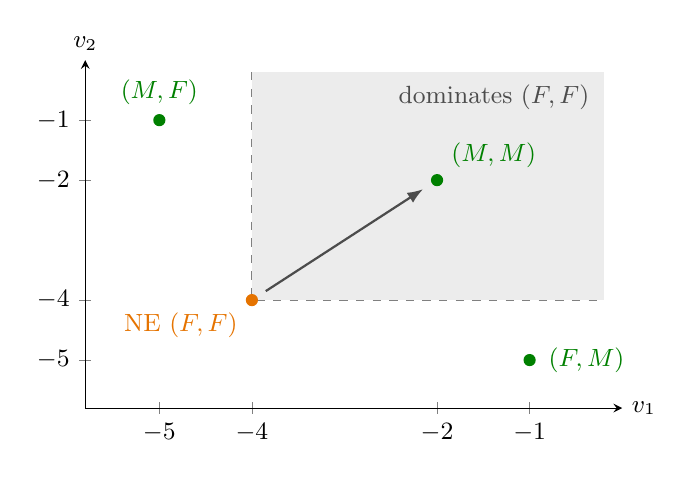
\begin{tikzpicture}[font=\small, >={Latex[length=2mm]}]
  \begin{axis}[
    axis lines=left, xmin=-5.8, xmax=0, ymin=-5.8, ymax=0,
    xtick={-5,-4,-2,-1}, ytick={-5,-4,-2,-1},
    xlabel={$v_1$}, ylabel={$v_2$},
    xlabel style={anchor=west, at={(axis description cs:1.0,0.0)}},
    ylabel style={rotate=-90, anchor=south, at={(axis description cs:0,1.0)}},
    width=8.4cm, height=6cm, clip=false]
    % region that Pareto dominates (F,F)
    \fill[gray!15] (axis cs:-4,-4) rectangle (axis cs:-0.2,-0.2);
    \draw[gray, dashed, thin] (axis cs:-4,-0.2) -- (axis cs:-4,-4) -- (axis cs:-0.2,-4);
    \node[gray!60!black, anchor=north east] at (axis cs:-0.25,-0.25) {dominates $(F,F)$};
    % Pareto improvement
    \draw[->, thick, gray!60!black] (axis cs:-3.85,-3.85) -- (axis cs:-2.15,-2.15);
    % profiles
    \fill[green!50!black] (axis cs:-2,-2) circle (2.2pt);
    \fill[green!50!black] (axis cs:-5,-1) circle (2.2pt);
    \fill[green!50!black] (axis cs:-1,-5) circle (2.2pt);
    \fill[orange!90!black] (axis cs:-4,-4) circle (2.2pt);
    \node[green!50!black, anchor=south west] at (axis cs:-1.95,-1.95) {$(M,M)$};
    \node[green!50!black, anchor=south] at (axis cs:-5,-0.9) {$(M,F)$};
    \node[green!50!black, anchor=west] at (axis cs:-0.9,-5) {$(F,M)$};
    \node[orange!90!black, anchor=north east] at (axis cs:-4.05,-4.05) {NE $(F,F)$};
  \end{axis}
\end{tikzpicture}
\end{document}
